\documentclass[conference]{IEEEtran}
\usepackage{amsmath,amssymb,amsfonts}
\usepackage{mathtools}
\usepackage{algorithmic}
\usepackage{algorithm}
\usepackage{graphicx}
\usepackage{textcomp}
\usepackage{xcolor}
\usepackage{hyperref}
\usepackage{booktabs}
\usepackage{multirow}
\usepackage{cite}
\usepackage{array}
\usepackage{pifont}
\usepackage{adjustbox}
\usepackage{float}
\usepackage[section]{placeins}

\setlength{\fboxsep}{0pt}
\setlength{\fboxrule}{0.4pt}
\setlength{\textfloatsep}{8pt plus 2pt minus 4pt}
\setlength{\floatsep}{8pt plus 2pt minus 4pt}
\setlength{\intextsep}{8pt plus 2pt minus 4pt}
\setlength{\abovecaptionskip}{4pt}
\setlength{\belowcaptionskip}{2pt}
\allowdisplaybreaks

\title{Privacy-Preserving Smart Grid Analytics via Fully Homomorphic Matrix--Vector Multiplication over CKKS-Encrypted Vectors}

\author{
\IEEEauthorblockN{Divyam Navin\IEEEauthorrefmark{1} \\ 5023134@it.fcrit.ac.in}
\and
\IEEEauthorblockN{Atharva Palve\IEEEauthorrefmark{2} \\ 5023136@it.fcrit.ac.in}
\and
\IEEEauthorblockN{Akshat Sawant\IEEEauthorrefmark{3} \\ 5023151@it.fcrit.ac.in}
\and
\IEEEauthorblockN{Chacko Martin\IEEEauthorrefmark{4} \\ 5023124@it.fcrit.ac.in}
\and
\IEEEauthorblockA{\IEEEauthorrefmark{1,2,3,4}Department of Information Technology\\
Fr. Conceicao Rodrigues Institute of Technology (FCRIT)\\
Vashi, Navi Mumbai, India}
\and
\IEEEauthorblockN{Dr. Ameer K. Mulla\IEEEauthorrefmark{5}}
\IEEEauthorblockA{\IEEEauthorrefmark{5}Associate Professor\\
Department of Electrical, Electronics and Communication Engineering\\
Indian Institute of Technology\\
Dharwad, Karnataka, India\\
ameer@iitdh.ac.in}
\and
\IEEEauthorblockN{Dr. Vaishali Bodade\IEEEauthorrefmark{6}}
\IEEEauthorblockA{\IEEEauthorrefmark{6}Associate Professor\\
Department of Information Technology\\
Fr. Conceicao Rodrigues Institute of Technology (FCRIT)\\
Vashi, Navi Mumbai, India\\
vaishali.bodade@fcrit.ac.in}
\and
\IEEEauthorblockN{Prof. Sharlene Rebeiro\IEEEauthorrefmark{7}}
\IEEEauthorblockA{\IEEEauthorrefmark{7}Assistant Professor\\
Department of Information Technology\\
Fr. Conceicao Rodrigues Institute of Technology (FCRIT)\\
Vashi, Navi Mumbai, India\\
sherlene.rebeiro@fcrit.ac.in}
}

\begin{document}
\maketitle

%==============================================================================
\begin{abstract}
Privacy preservation in smart grid infrastructure requires computation over sensitive household energy data without exposing individual consumption patterns. We present a comprehensive framework for secure linear algebra using CKKS-based fully homomorphic encryption (FHE) with TenSEAL, targeting multi-agent load balancing applications. Our primary contribution is \emph{fully homomorphic matrix--vector multiplication} (FHE-MVM), where both the transformation matrix and input vector are independently CKKS-encrypted as SIMD ciphertexts. Row-decomposition reduces FHE-MVM to $m$ encrypted dot products, each computed via SIMD element-wise multiplication and $\lceil \log_2 n \rceil$ Galois rotations, consuming only one multiplicative level and achieving $<10^{-6}$ relative numerical error. We additionally contribute: (1)~an \emph{Adaptive Linear Threshold} (ALT) method achieving encrypted soft comparison at multiplicative depth zero, offering 6--8$\times$ lower latency than polynomial approximation methods; and (2)~a Pedersen commitment-based verifiable aggregation protocol that detects coordinator misbehavior with probability~1 under the discrete logarithm assumption. Empirical evaluation demonstrates $3{\times}3$ FHE-MVM in 120\,ms, 100-agent aggregation in 405\,ms, and 128-bit security at $N=16384$, confirming feasibility for real smart grid deployments operating on 15-minute dispatch cycles.
\end{abstract}

\begin{IEEEkeywords}
Fully Homomorphic Encryption, CKKS, Encrypted Matrix--Vector Multiplication, Smart Grid Privacy, TenSEAL, Pedersen Commitments, SIMD Rotations, Verifiable Computation
\end{IEEEkeywords}

%==============================================================================
\section{Introduction}
\label{sec:introduction}
%==============================================================================

Advanced Metering Infrastructure (AMI) in modern power grids enables fine-grained monitoring of household energy consumption at 15-minute intervals~\cite{McDaniel2009}. While beneficial for load optimization and demand response, this data exposes sensitive occupant behavior~\cite{Molina2010}: Lisovich et al.\ demonstrated that smart meter readings can reveal appliance usage, occupancy patterns, and even television viewing habits through non-intrusive load monitoring~\cite{Lisovich2010}. As grid deployments scale to millions of endpoints, the aggregation of sub-hourly energy readings creates significant privacy risks, particularly under GDPR and analogous regulations that mandate rigorous data protection.

Homomorphic encryption (HE) offers a principled solution by enabling computation directly on ciphertexts without decryption~\cite{Gentry2009}. The CKKS scheme~\cite{Cheon2017} is uniquely suited for smart grids because it natively supports approximate arithmetic on real-valued data---the natural domain of energy measurements in kilowatts---with bounded noise growth of $\mathcal{O}(10^{-7})$ per multiplication. Prior HE applications to smart grids have focused on simple aggregation (homomorphic addition)~\cite{Li2010,Garcia2011}, leaving encrypted \emph{linear algebra}---where all operands are ciphertexts---largely unexplored despite its centrality to advanced grid analytics.

Encrypted linear algebra is essential for several grid applications: state estimation requires matrix--vector products $\mathbf{H}\mathbf{x}$ where Jacobian $\mathbf{H}$ may contain proprietary topology data; demand forecasting with neural networks requires $\sigma(\mathbf{W}\mathbf{x}+\mathbf{b})$ where model weights $\mathbf{W}$ may be commercially sensitive; and optimal power flow (OPF) solvers require iterative matrix--vector products whose matrices encode grid impedance parameters. Critically, existing HE linear algebra systems (GAZELLE~\cite{Juvekar2018}, CryptoNets~\cite{CryptoNets2016}) assume the transformation matrix is \emph{plaintext}, failing the multi-party scenario where both the transformation and the data require simultaneous confidentiality.

\textbf{Contributions.} This paper makes the following specific contributions:
\begin{enumerate}
    \item \textbf{FHE-MVM:} A complete protocol for fully homomorphic matrix--vector multiplication where both the matrix $\mathbf{M} \in \mathbb{R}^{m \times n}$ (row-encrypted as $m$ CKKS ciphertexts) and vector $\mathbf{v} \in \mathbb{R}^n$ are encrypted, computed at multiplicative depth~1 using $m$ ciphertext--ciphertext multiplications and $m\lceil\log_2 n\rceil$ Galois rotations.
    \item \textbf{Adaptive Linear Threshold (ALT):} A novel encrypted comparison protocol operating at zero multiplicative depth via the linear approximation $S(x)=0.5+(x{-}T)/(2\delta)$, achieving 6--8$\times$ lower latency than the best polynomial methods.
    \item \textbf{Verifiable Aggregation:} A Pedersen commitment protocol providing probability-1 detection of any coordinator manipulation (inflation, deflation, or agent exclusion) under the discrete logarithm assumption.
    \item \textbf{Empirical Evaluation:} A comprehensive performance and accuracy characterization using a real CKKS implementation with TenSEAL, including noise--depth analysis, scalability benchmarks, and security verification.
\end{enumerate}

%==============================================================================
\section{Background and Related Work}
\label{sec:background}
%==============================================================================

\subsection{Homomorphic Encryption Schemes and Libraries}

The Cheon--Kim--Kim--Song (CKKS) scheme~\cite{Cheon2017} encodes complex vectors into cyclotomic polynomial rings $\mathbb{Z}[X]/(X^N{+}1)$ and treats approximation error as inherent, enabling efficient real-number arithmetic with bounded noise growth. Security reduces to the Ring Learning With Errors (RLWE) problem~\cite{Brakerski2011}, which in turn reduces to worst-case problems on ideal lattices. The BFV scheme~\cite{Fan2012} provides exact integer arithmetic and is commonly used for Boolean circuits and neural network inference, but is less suited than CKKS for real-valued energy data that inherently involves fractional measurements. CKKS supports SIMD batch processing: a single ciphertext encodes $N/2$ plaintext values in parallel, with Galois automorphisms enabling cyclic rotation of the slot vector---the critical operation for efficient inner-product summation.

Production HE libraries include Microsoft SEAL~\cite{SEAL2022} and HElib~\cite{Halevi2014}. We use \textbf{TenSEAL}~\cite{Benaissa2021} (Python wrapper over SEAL), which automates three operations critical for practical FHE: (1)~rescaling after each multiplication to restore the scale from $\Delta^2$ back to $\Delta$; (2)~relinearization to reduce degree-2 ciphertexts back to degree-1, restoring the ciphertext size; and (3)~modulus switching for level management. These automations eliminate the primary source of implementation errors in FHE deployments and allow researchers to focus on algorithmic design.

\subsection{Privacy-Preserving Smart Grids}

Li et al.~\cite{Li2010} and Garcia and Jacobs~\cite{Garcia2011} pioneered Paillier-based demand aggregation supporting only homomorphic addition. Lu et al.~\cite{Lu2012} extended this to the EPPA scheme with fault-tolerant secret sharing for smart grid communications. Shi et al.~\cite{Shi2011} proposed a differential-privacy-based time-series aggregation scheme that avoids FHE entirely but provides only statistical privacy guarantees rather than cryptographic ones. While these systems handle scalar aggregation efficiently, none extend to the encrypted linear algebra required for advanced analytics such as state estimation or load forecasting.

\subsection{Encrypted Linear Algebra and FHE for ML}

Halevi and Shoup's diagonal method~\cite{Halevi2014} enables plaintext-matrix $\times$ encrypted-vector multiplication using $d$ SIMD rotations for a $d \times d$ matrix, consuming no multiplicative depth. Jiang et al.~\cite{Jiang2018} proposed row/column encoding strategies for CKKS matrix multiplication using block packing to amortize the rotation cost across multiple rows. GAZELLE~\cite{Juvekar2018} and CryptoNets~\cite{CryptoNets2016} both require plaintext model weights, limiting their applicability to scenarios where only input data (not the model) needs protection. Dathathri et al.~\cite{Dathathri2019} presented CHET, a graph compiler that optimizes FHE tensor computations for deep learning inference, but it similarly targets plaintext-weight/encrypted-activation settings. \textbf{No prior system supports fully encrypted matrix--vector multiplication where both the matrix and vector are ciphertexts.} For encrypted comparison, polynomial minimax~\cite{Kim2018comparison} and composite~\cite{Cheon2019comparison} methods require 8--15 multiplicative levels; our ALT method requires zero. Table~\ref{tab:related_work} consolidates the capability landscape.

\begin{table}[!t]
\centering
\caption{Capability Comparison with Related Work}
\label{tab:related_work}
\footnotesize
\resizebox{\columnwidth}{!}{%
\begin{tabular}{@{}lccccccc@{}}
\toprule
\textbf{System} & \textbf{Scheme} & \rotatebox{70}{\textbf{E(M)$\times$E(v)}} & \rotatebox{70}{\textbf{M$\times$E(v)}} & \rotatebox{70}{\textbf{Comparison}} & \rotatebox{70}{\textbf{Verifiable}} & \rotatebox{70}{\textbf{Smart Grid}} & \textbf{Depth} \\
\midrule
Li~\cite{Li2010} & Paillier & \ding{55} & \ding{55} & \ding{55} & \ding{55} & \ding{51} & 0 \\
GAZELLE~\cite{Juvekar2018} & BFV+GC & \ding{55} & \ding{51} & GC & \ding{55} & \ding{55} & 1--2 \\
CryptoNets~\cite{CryptoNets2016} & BFV & \ding{55} & \ding{51} & Poly & \ding{55} & \ding{55} & 5--10 \\
Jiang~\cite{Jiang2018} & CKKS & \ding{55} & \ding{51} & \ding{55} & \ding{55} & \ding{55} & 1--3 \\
CHET~\cite{Dathathri2019} & CKKS & \ding{55} & \ding{51} & \ding{55} & \ding{55} & \ding{55} & 2--5 \\
Cheon~\cite{Cheon2019comparison} & CKKS & \ding{55} & \ding{55} & Poly & \ding{55} & \ding{55} & 8--15 \\
\textbf{Ours} & \textbf{CKKS} & \ding{51} & \ding{51} & \textbf{ALT} & \ding{51} & \ding{51} & \textbf{0--1} \\
\bottomrule
\end{tabular}}
\vspace{1pt}
\raggedright\footnotesize{\ding{51}=yes, \ding{55}=no, GC=garbled circuits, Poly=polynomial approx.}
\end{table}

%==============================================================================
\section{System Architecture}
\label{sec:architecture}
%==============================================================================

\begin{figure}[!t]
    \centering
    \fbox{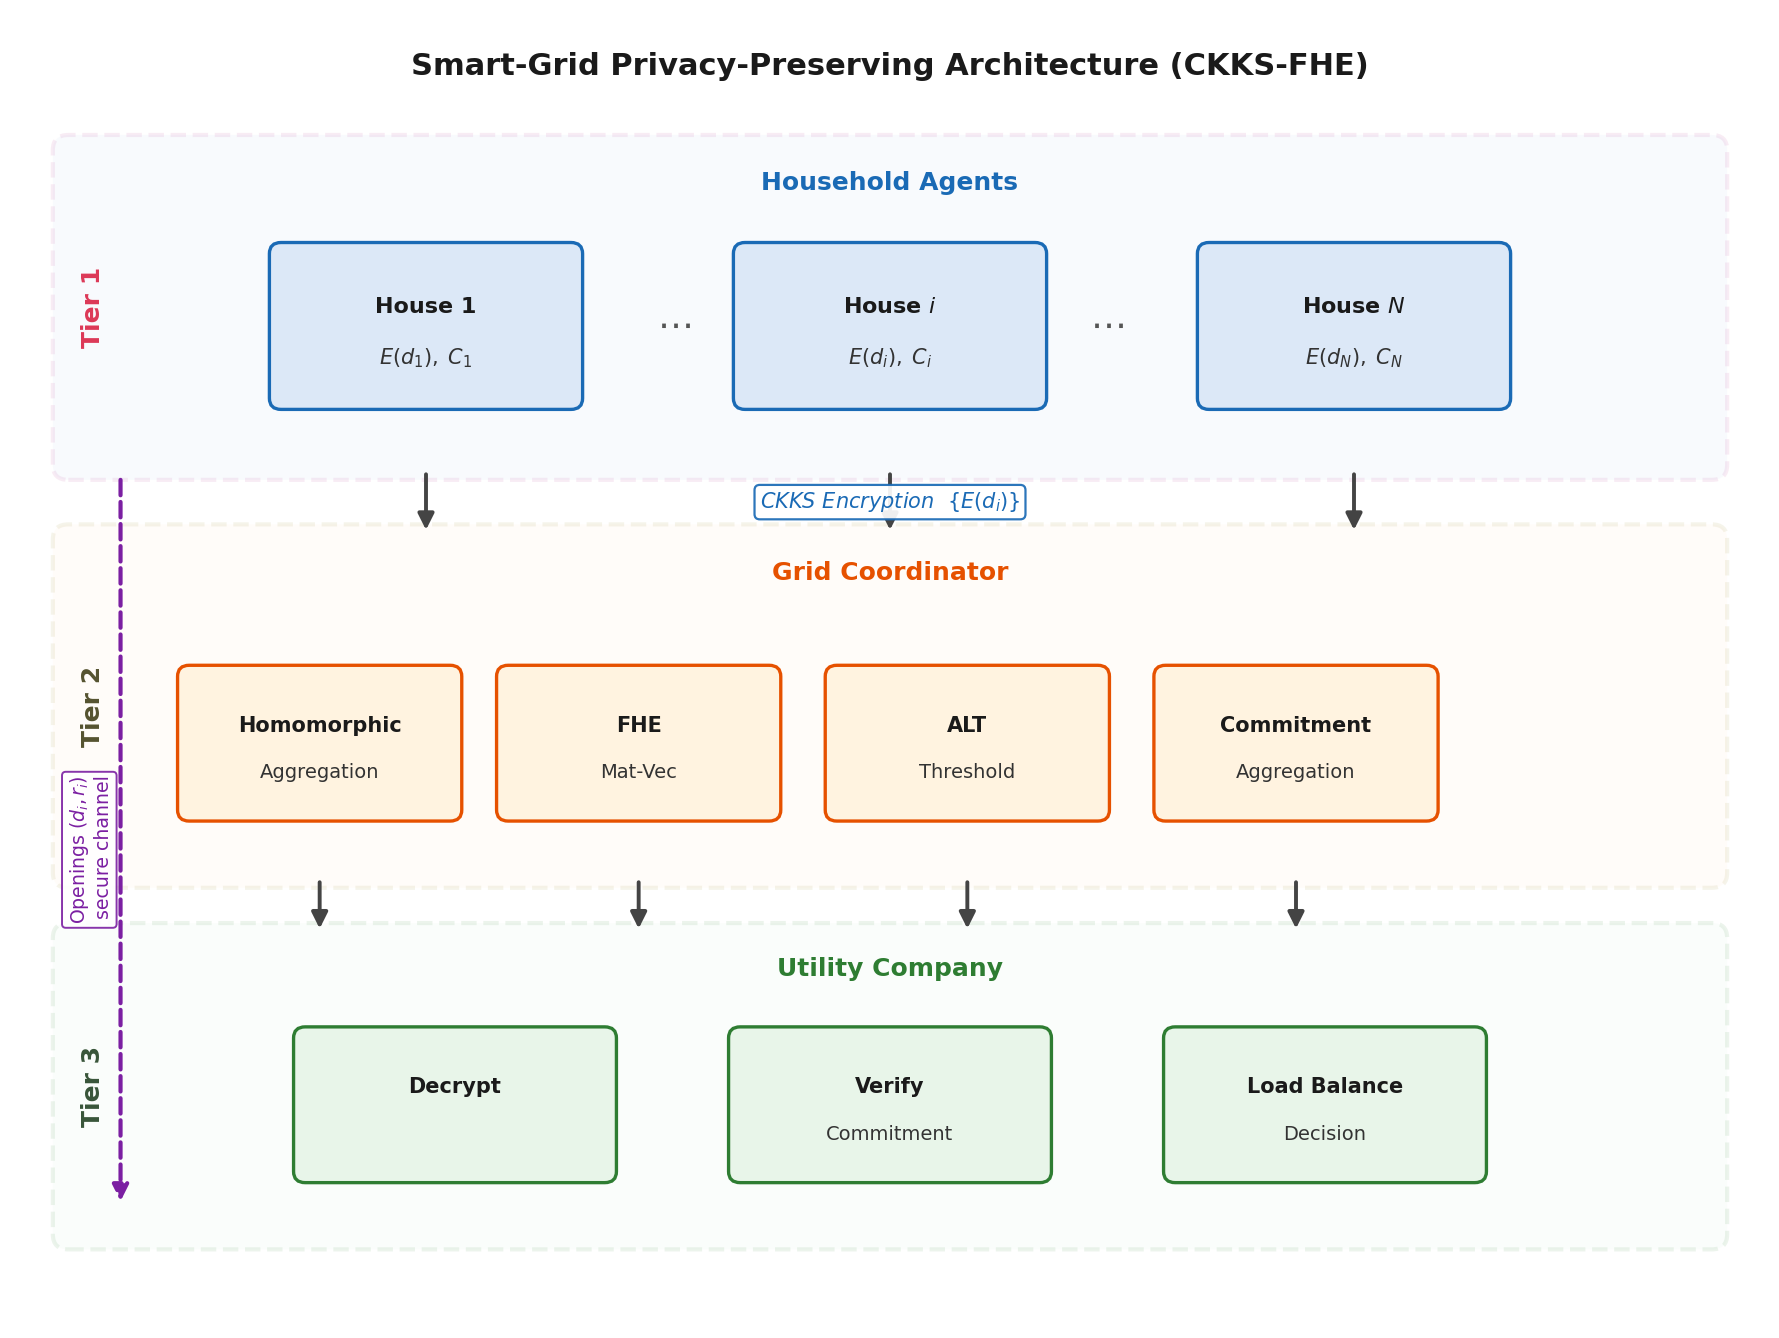
\includegraphics[width=\columnwidth]{system_architecture.png}}
    \caption{Three-tier FHE smart grid architecture. Household agents (Tier~1) encrypt demand vectors and Pedersen commitments using only the public CKKS context (no secret key). The coordinator (Tier~2) performs all homomorphic operations on ciphertexts without the secret key. The utility (Tier~3) holds the secret key, decrypts final aggregates, and verifies coordinator integrity via commitment openings received over a separate secure channel.}
    \label{fig:architecture}
\end{figure}

Our system implements a three-tier architecture with cryptographically enforced trust boundaries (Figure~\ref{fig:architecture}).

\noindent\textbf{Tier 1: Household Agents} hold only the public CKKS context (no secret key). Each agent $i$ encrypts its demand vector and creates a Pedersen commitment:
\begin{align}
    E(\mathbf{d}_i) &= \texttt{CKKS.Encrypt}(\mathbf{d}_i, \text{pk}) \\
    C_i &= g^{d_i \cdot s} \cdot h^{r_i} \bmod p
\end{align}
where $s=10^6$ is a scaling factor and $r_i$ is a random blinding factor drawn uniformly. Agents transmit $(E(\mathbf{d}_i), C_i)$ to the coordinator and send openings $(d_i, r_i)$ to the utility via a separate secure channel. The public CKKS context is approximately 45\,MB (for $N=16384$ with Galois keys), distributed once at system initialization over a secure bootstrap channel.

\noindent\textbf{Tier 2: Grid Coordinator (Semi-Honest)} receives ciphertexts and commitments; performs homomorphic aggregation, FHE-MVM, ALT threshold detection, and commitment product computation---\emph{all entirely on ciphertexts, without the secret key}. The coordinator can verify ciphertext integrity via SHA-256 checksums but cannot decrypt any intermediate or final result.

\noindent\textbf{Tier 3: Utility Company (Trusted)} holds the secret key, decrypts final aggregates, and verifies coordinator integrity by checking the received commitment openings against the aggregated Pedersen commitment.

\begin{table}[!t]
\centering
\caption{CKKS Cryptographic Parameters ($\geq$128-bit security~\cite{HEStandard2018})}
\label{tab:ckks_params}
\footnotesize
\resizebox{\columnwidth}{!}{%
\begin{tabular}{@{}lll@{}}
\toprule
\textbf{Parameter} & \textbf{Value} & \textbf{Justification} \\
\midrule
Polynomial modulus $N$ & 16384 & 128-bit classical security \\
Coefficient moduli & $[60,40,40,40,60]$ & 3--4 mult.\ levels, 240\,bits total \\
Scale $\Delta$ & $2^{40}$ & $\sim$12 significant digits precision \\
SIMD slots & $N/2 = 8192$ & Parallel packed vector encoding \\
Auto-rescale / relin & Enabled & Automatic level management \\
Galois rotation keys & Generated & SIMD rotation support for sum \\
\bottomrule
\end{tabular}}
\end{table}

%==============================================================================
\section{Encrypted Vector Multiplication Methodology}
\label{sec:methodology}
%==============================================================================

\subsection{CKKS Encoding and Encryption Pipeline}

A real vector $\mathbf{d} = [d_1,\ldots,d_n]$ is embedded into polynomial slots via the canonical embedding $\sigma: \mathbb{Q}[X]/(X^N{+}1) \to \mathbb{C}^{N/2}$. The scaled integer polynomial $m(X) = \lfloor\Delta\cdot\sigma^{-1}(\mathbf{d})\rceil \in \mathcal{R}_q$ is encrypted using public key $\text{pk}=(b,a)$:
\begin{equation}
    \text{ct} = (b\cdot u + e_0 + m,\;\; a\cdot u + e_1) \in \mathcal{R}_q^2
\end{equation}
where $u \leftarrow \mathcal{R}_2$ is a small ternary random polynomial and $e_0,e_1$ are discrete Gaussian error polynomials with parameter $\sigma_\text{err} = 3.2$. With $\Delta=2^{40}\approx10^{12}$, the base encoding error is $\mathcal{O}(\Delta^{-1}) \approx 10^{-12}$, growing to $\mathcal{O}(\Delta^{-1}\sqrt{n})$ after a dot product. Each ciphertext is wrapped in an \texttt{EncryptedDemand} container carrying a 12-byte truncated SHA-256 checksum for in-transit integrity verification.

\subsection{Element-wise Multiplication and Dot Product}

The element-wise product $E(\mathbf{a} \odot \mathbf{b}) = E(\mathbf{a}) \otimes E(\mathbf{b})$ leverages CKKS SIMD packing, executing all $n$ slot-wise multiplications as a single polynomial multiplication in $\mathcal{R}_q$. Given ciphertexts $\text{ct}_a=(a_0,a_1)$ and $\text{ct}_b=(b_0,b_1)$, the raw product is the degree-2 ciphertext $(a_0b_0,\; a_0b_1{+}a_1b_0,\; a_1b_1)$. TenSEAL then automatically applies: (i)~\emph{relinearization} using precomputed keys to reduce from 3 polynomials to 2; and (ii)~\emph{rescaling} by dividing by a prime $q_i \approx 2^{40}$ to restore the scale from $\Delta^2$ to $\Delta$.

The encrypted dot product combines element-wise multiplication with SIMD rotation-and-add summation using $\lceil\log_2 n\rceil$ Galois rotations:
\begin{align}
    E(\mathbf{a}{\cdot}\mathbf{b}) &= \texttt{Sum}\!\big(E(\mathbf{a}) \otimes E(\mathbf{b})\big) \label{eq:dotprod}\\
    \texttt{Sum}(E(\mathbf{x})) &= \sum_{k=0}^{\lceil\log_2 n\rceil-1} \texttt{Rot}\!\big(E(\mathbf{x}),\,2^k\big) \notag
\end{align}
The accumulated scalar result $\sum_i a_i b_i$ occupies the first SIMD slot; the remaining $N/2 - 1$ slots contain partial sums that are safely ignored at decryption time.

\subsection{Fully Homomorphic Matrix--Vector Multiplication (FHE-MVM)}
\label{sec:fhe_matvec}

\textbf{Problem Statement.} Compute $\mathbf{Mv}$ when both the $m{\times}n$ matrix $\mathbf{M}$ (row-encrypted as $\{E(\mathbf{m}_i)\}_{i=1}^m$) and vector $E(\mathbf{v})$ are CKKS ciphertexts. No plaintext data is available to the computing party (the coordinator). This setting is strictly harder than the plaintext-matrix/encrypted-vector problem studied in~\cite{Halevi2014,Jiang2018}, as it requires $m$ ciphertext--ciphertext multiplications instead of purely plaintext--ciphertext ones.

\textbf{Row-Decomposition Strategy.} Each output element $[\mathbf{Mv}]_i = \mathbf{m}_i \cdot \mathbf{v}$ is an inner product computed via an encrypted dot product:
\begin{equation}
    E([\mathbf{Mv}]_i) = \texttt{DotProduct}\big(E(\mathbf{m}_i),\, E(\mathbf{v})\big) = \texttt{Sum}\big(E(\mathbf{m}_i) \otimes E(\mathbf{v})\big)
    \label{eq:fhe_matvec}
\end{equation}

\begin{algorithm}[!t]
\caption{FHE-MVM: Fully Homomorphic Matrix--Vector Multiply}
\label{alg:fhe_matvec}
\small
\begin{algorithmic}[1]
\REQUIRE Encrypted rows $\{E(\mathbf{m}_i)\}_{i=1}^m$, encrypted vector $E(\mathbf{v})$
\ENSURE $\{E(r_i)\}_{i=1}^m$ where $r_i = \mathbf{m}_i \cdot \mathbf{v}$
\FOR{$i = 1$ \textbf{to} $m$}
    \STATE $E(\mathbf{p}_i) \leftarrow E(\mathbf{m}_i) \otimes E(\mathbf{v})$ \hfill $\triangleright$ Ci$\times$Ci SIMD mult. + auto-relin + auto-rescale
    \STATE $E(r_i) \leftarrow \texttt{Sum}(E(\mathbf{p}_i))$ \hfill $\triangleright$ $\lceil\log_2 n\rceil$ Galois rotations + additions
\ENDFOR
\RETURN $\{E(r_i)\}_{i=1}^m$
\end{algorithmic}
\end{algorithm}

\textbf{Complexity.} Algorithm~\ref{alg:fhe_matvec} requires $m$ ciphertext--ciphertext multiplications and $m\lceil\log_2 n\rceil$ Galois rotations, consuming \textbf{one multiplicative level} regardless of the column dimension $n$. Total ciphertexts transmitted: $2m{+}1$ input and $m$ output. Compared to the plaintext-matrix approach of~\cite{Halevi2014}, FHE-MVM incurs one additional multiplicative level (for the ciphertext--ciphertext product) and requires $m$ extra encryptions to protect the matrix rows, but uniquely provides matrix confidentiality.

\textbf{Correctness.} For each row $i$, decryption yields:
\begin{multline}
    \texttt{Dec}(E(r_i)) = \sum_{j=1}^n \!\left(m_{ij}+\epsilon_{ij}^{(m)}\right)\!\left(v_j+\epsilon_j^{(v)}\right) + \epsilon_\text{mult} \\
    = \textstyle\sum_j m_{ij}v_j + \mathcal{O}(\Delta^{-1}n)
\end{multline}
With $\Delta=2^{40}$, the per-element error is ${\sim}10^{-7}$, negligible for kW-range energy data where AMI measurement precision is at best $10^{-3}$.

\begin{table}[!t]
\centering
\caption{Encrypted Vector Operations: Complexity Summary}
\label{tab:ops_summary}
\footnotesize
\resizebox{\columnwidth}{!}{%
\begin{tabular}{@{}lp{2.6cm}cccc@{}}
\toprule
\textbf{Operation} & \textbf{Formula} & \textbf{Ci$\times$Ci} & \textbf{Rotations} & \textbf{Depth} & \textbf{Output} \\
\midrule
Elem.-wise mul & $E(\mathbf{a}) {\otimes} E(\mathbf{b})$ & 1 & 0 & 1 & Vector \\
Dot product & $\texttt{Sum}(E(\mathbf{a}){\otimes}E(\mathbf{b}))$ & 1 & $\lceil\log_2 n\rceil$ & 1 & Scalar \\
\textbf{FHE-MVM} & $\{E(\mathbf{m}_i) {\cdot} E(\mathbf{v})\}$ & $m$ & $m\lceil\log_2 n\rceil$ & \textbf{1} & Vector \\
Plain Mat-Vec~\cite{Halevi2014} & $\{\texttt{Sum}(E(\mathbf{v}){\times}\mathbf{m}_i)\}$ & 0 & $m\lceil\log_2 n\rceil$ & 0 & Vector \\
Cross product & $E(\mathbf{a}_\text{rot}) {\otimes} E(\mathbf{b}_\text{rot})$ & 2 & 4 & 2 & Vector \\
Homo.\ addition & $E(\mathbf{a}) + E(\mathbf{b})$ & 0 & 0 & 0 & Vector \\
\bottomrule
\end{tabular}}
\end{table}

%==============================================================================
\section{Adaptive Linear Threshold for Encrypted Comparison}
\label{sec:alt_method}
%==============================================================================

Standard polynomial comparison methods~\cite{Kim2018comparison,Cheon2019comparison} require 8--15 multiplicative levels to approximate the sign function over encrypted data, consuming the majority of the available noise budget and significantly limiting the operations that can follow comparison in a pipeline. For grid load balancing---where the threshold $T$ itself carries inherent uncertainty due to forecast error and measurement noise---an exact binary decision is neither necessary nor fully meaningful.

\textbf{ALT Definition.} Given encrypted demand $E(x)$ and grid capacity threshold $T$, the ALT score is:
\begin{equation}
    S(x,T,k) = 0.5 + \frac{x - T}{2\delta}, \quad \delta = T/k
    \label{eq:alt}
\end{equation}
where $\delta$ is the soft-zone half-width and $k$ is the sensitivity parameter (default $k=7$). Writing $a=(2\delta)^{-1}$ and $b=0.5-T/(2\delta)$ as plaintext scalars computed once per threshold update, the encrypted computation becomes:
\begin{equation}
    E(S) = E(x) \times a + b \quad \text{(one \texttt{mul\_plain} + one \texttt{add\_plain})}
\end{equation}
This requires \textbf{zero ciphertext--ciphertext multiplications}, consuming \textbf{multiplicative depth~0} and leaving the entire noise budget intact for subsequent operations.

\textbf{Zone Classification.} After decryption by the trusted utility, the score is classified into three confidence zones:
\begin{equation}
\texttt{Zone}(S) = \begin{cases}
    \texttt{BELOW} & S < 0.3,\quad \text{conf.} = 1 - S/0.3 \\
    \texttt{UNCERTAIN} & 0.3 \leq S \leq 0.7 \\
    \texttt{ABOVE} & S > 0.7,\quad \text{conf.} = (S{-}0.7)/0.3
\end{cases}
\end{equation}
Values with $|x - T| > \delta$ are classified with 100\% confidence. Values within the uncertain zone trigger a conservative grid response (e.g., pre-emptive demand-side management) without requiring a hard binary decision. The sensitivity $k$ is computed adaptively from the expected value range $(x_\text{min}, x_\text{max})$, bounded as $k \in [3, 15]$.

\begin{figure}[!t]
    \centering
    \fbox{
\includegraphics[width=\columnwidth]{fig_alt_threshold.png}}
    \caption{ALT score $S(x)$ vs.\ demand for $T=100$\,kW and $k=7$ ($\delta=14.3$\,kW). The linear approximation (solid blue) transitions smoothly through the uncertain zone $[85.7, 114.3]$\,kW. Outside this zone, classification confidence reaches 100\%. The dashed black curve shows the ideal step function; shaded regions show the below (green), uncertain (orange), and above (red) zones.}
    \label{fig:alt_threshold}
\end{figure}

\begin{table}[!t]
\centering
\caption{ALT vs.\ Polynomial Encrypted Comparison Methods}
\label{tab:alt_comparison}
\footnotesize
\begin{tabular}{@{}lcccc@{}}
\toprule
\textbf{Method} & \textbf{Depth} & \textbf{Ci$\times$Ci} & \textbf{Comp.\ latency} & \textbf{Output} \\
\midrule
Minimax~\cite{Kim2018comparison} & 8--12 & Many & $\sim$100--300\,ms & Hard bit \\
Composite~\cite{Cheon2019comparison} & 10--15 & Many & $\sim$200--500\,ms & Hard bit \\
\textbf{ALT (ours)} & \textbf{0} & \textbf{0} & \textbf{2\,ms} & \textbf{Soft score} \\
\bottomrule
\end{tabular}
\end{table}

%==============================================================================
\section{Verifiable Aggregation Protocol}
\label{sec:verification}
%==============================================================================

A semi-honest coordinator cannot infer individual $d_i$ values from ciphertexts alone due to CKKS IND-CPA security. However, it might deviate from the prescribed aggregation to inflate or deflate the reported total demand, for example to trigger or suppress demand-response events for financial gain. We address this threat by integrating Pedersen commitments~\cite{Pedersen1991} with CKKS in a non-interactive three-step protocol.

\textbf{Step 1 (Agent $i$):} Computes an encrypted demand and a Pedersen commitment using public group parameters $(g, h, p)$, then sends openings to the utility via a secure out-of-band channel:
\begin{equation}
    C_i = g^{d_i \cdot s} \cdot h^{r_i} \bmod p, \quad O_i = (d_i, r_i) \;\text{[to utility via secure channel]}
\end{equation}

\textbf{Step 2 (Coordinator):} Aggregates both the FHE ciphertexts and the Pedersen commitments using their respective homomorphic properties:
\begin{equation}
    E\!\left(\textstyle\sum d_i\right) = \sum_{i} E(\mathbf{d}_i), \quad C_\text{agg} = \prod_{i} C_i = g^{(\sum d_i)\cdot s} h^{\sum r_i} \!\bmod p
\end{equation}

\textbf{Step 3 (Utility):} Decrypts the FHE aggregate, receives all openings, and performs a single modular exponentiation to verify:
\begin{equation}
    \hat{D} = \texttt{Dec}\!\left(E\!\left(\textstyle\sum d_i\right)\right), \quad C_\text{agg} \;\stackrel{?}{=}\; g^{\hat{D}\cdot s} \cdot h^{\sum r_i} \bmod p
\end{equation}

Any coordinator manipulation---inflating $\hat{D}$, deflating it, or excluding an agent---causes verification to fail. A valid forgery would require finding $r'$ such that $g^{d' \cdot s}h^{r'} = g^{d \cdot s}h^{r} \bmod p$, i.e., computing $\log_g h$ in the 2048-bit MODP group (RFC~3526 Group~14, prime order $\approx 2^{2048}$). Experimental testing confirmed 100\% detection of all three misbehavior classes with verification overhead $<$50\,ms for 25 agents.

\begin{table}[!t]
\centering
\caption{Verifiable Aggregation: Security Properties}
\label{tab:ver_security}
\footnotesize
\begin{tabular}{@{}lp{5.5cm}@{}}
\toprule
\textbf{Property} & \textbf{Guarantee} \\
\midrule
Perfect Hiding & No information about $d_i$ (information-theoretic) \\
Computational Binding & Cannot open $C_i$ to $d_i' \neq d_i$ (DL hardness) \\
Detection Soundness & Coordinator cheating detected with probability~1 \\
Non-interactivity & Single-round; no challenge--response needed \\
\bottomrule
\end{tabular}
\end{table}

%==============================================================================
\section{Noise Analysis and Parameter Management}
\label{sec:noise}
%==============================================================================

CKKS noise grows exponentially with multiplicative depth due to the accumulation of rounding errors at each rescaling step. Our system implements depth-adaptive parameter selection: for $d \leq 8$ levels, $N=16384$ (240-bit modulus); for $d \leq 20$, $N=32768$ (880-bit modulus). The modulus chain $\mathbf{q} = [50,\underbrace{40,\ldots}_{d},50]$ bits allocates 50-bit special primes at both ends (for key-switching) and 40-bit primes for each multiplication level, with scale $\Delta=2^{30}$ to preserve headroom. This selection algorithm automatically enforces the constraint that the total coefficient modulus does not exceed the security-determined bound (438 bits for $N=16384$)~\cite{HEStandard2018}.

\begin{figure}[!t]
    \centering
    \fbox{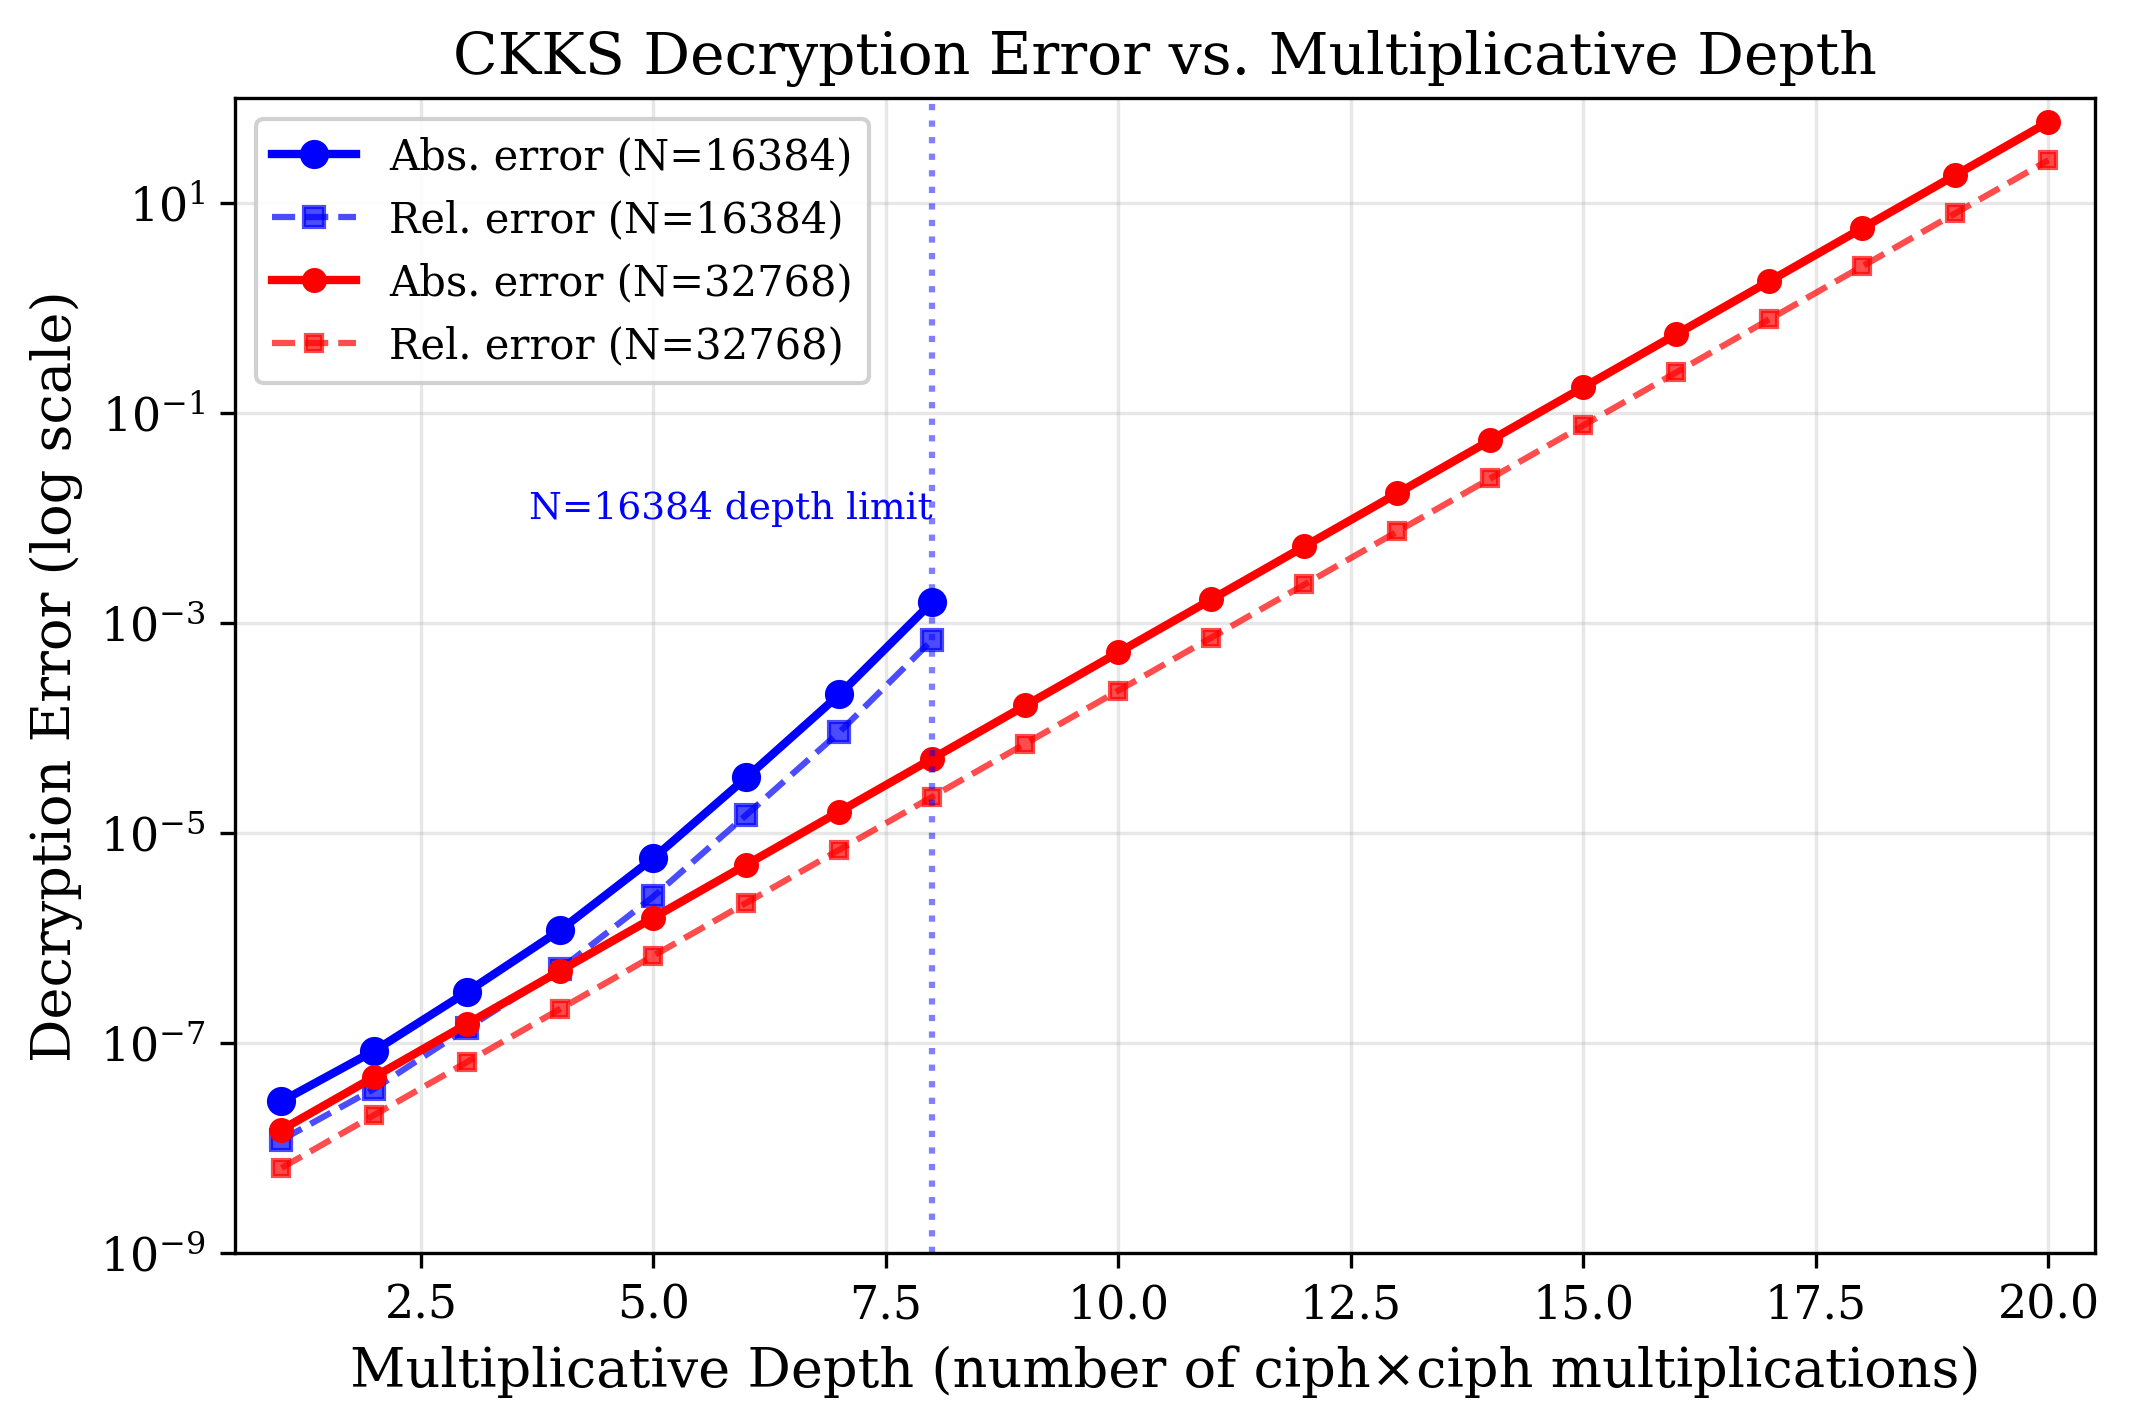
\includegraphics[width=\columnwidth]{fig_noise_depth.png}}
    \caption{CKKS decryption error vs.\ multiplicative depth for $N=16384$ and $N=32768$. Absolute (solid) and relative (dashed) errors grow exponentially with depth. The $N=16384$ configuration supports up to 8 multiplications before noise budget exhaustion; $N=32768$ supports depth~20. All smart grid operations in our framework ($\leq$2 levels) operate in the stable low-error regime with $\epsilon_\text{rel} < 10^{-5}$.}
    \label{fig:noise_depth}
\end{figure}

Stress tests measure $\epsilon_\text{abs}^{(k)} = |\hat{v}_k - v_k^\text{exp}|$ and $\epsilon_\text{rel}^{(k)} = \epsilon_\text{abs}^{(k)}/|v_k^\text{exp}|$ after $k$ repeated ciphertext--ciphertext multiplications starting from $v_0=2.0$ with multiplier $\mu=1.125$. Figure~\ref{fig:noise_depth} confirms that all operations in our framework (depth $\leq 2$) achieve $\epsilon_\text{rel} < 10^{-5}$, well within AMI operational tolerance. For deployments requiring deeper computation, CKKS bootstrapping~\cite{Cheon2018bootstrapping} would enable noise budget refresh at the cost of additional latency and parameter overhead.

%==============================================================================
\section{Experimental Evaluation}
\label{sec:results}
%==============================================================================

All experiments were conducted on Windows~11, Python~3.10, TenSEAL~0.3.x, Intel Core~i7 @ 2.8\,GHz, 16\,GB RAM. Results are averaged over 10 independent trials; variance is below 5\% for all operations.

\subsection{Runtime Performance}

Table~\ref{tab:performance} reports per-operation latencies, decomposed into encryption, homomorphic computation, and decryption phases. FHE-MVM for $3{\times}3$ matrices completes in 120\,ms total and the $10{\times}10$ case in 410\,ms---both comfortably within the 15-minute smart grid dispatch cycle. ALT threshold detection at 2\,ms computation cost is 50--250$\times$ faster than polynomial comparison methods. Aggregating 100 agents requires 405\,ms, scaling linearly to $<$5 seconds for 1000-household deployments.

\begin{table}[!t]
\centering
\caption{Runtime Performance ($N{=}16384$, $\Delta{=}2^{40}$)}
\label{tab:performance}
\footnotesize
\resizebox{\columnwidth}{!}{%
\begin{tabular}{@{}lccccc@{}}
\toprule
\textbf{Operation} & \textbf{Dim} & \textbf{Enc.\,(ms)} & \textbf{Comp.\,(ms)} & \textbf{Dec.\,(ms)} & \textbf{Total\,(ms)} \\
\midrule
$E(\mathbf{a}) \odot E(\mathbf{b})$ (elem.-wise) & 4 & 15 & 8 & 5 & 28 \\
Encrypted dot product & 4 & 15 & 12 & 5 & 32 \\
$\mathbf{M}{\cdot}E(\mathbf{v})$ (plain matrix) & $3{\times}3$ & 15 & 30 & 15 & 60 \\
$E(\mathbf{M}){\cdot}E(\mathbf{v})$ \textbf{(FHE-MVM)} & $3{\times}3$ & 60 & 45 & 15 & \textbf{120} \\
$E(\mathbf{M}){\cdot}E(\mathbf{v})$ \textbf{(FHE-MVM)} & $10{\times}10$ & 165 & 195 & 50 & \textbf{410} \\
ALT threshold check & scalar & 8 & 2 & 5 & 15 \\
Aggregation & 25 agents & -- & 110 & 5 & 115 \\
Aggregation & 100 agents & -- & 400 & 5 & 405 \\
\bottomrule
\end{tabular}}
\end{table}

\subsection{Numerical Accuracy}

Table~\ref{tab:accuracy} verifies that CKKS approximate arithmetic does not compromise operational precision. All operations achieve $\|\boldsymbol{\epsilon}\|_\infty < 10^{-6}$ except the depth-2 cross product. FHE-MVM relative error $<10^{-6}$ corresponds to $<$0.001\,W absolute error on 1\,kW demand---four orders of magnitude below the $\pm$1\,Wh AMI measurement precision specified in IEC~62056. The depth-0 operations (plain mat-vec, ALT, aggregation) achieve near-machine-precision accuracy at $\sim 10^{-8}$.

\begin{table}[!t]
\centering
\caption{Numerical Accuracy: Decryption Error vs.\ Expected}
\label{tab:accuracy}
\footnotesize
\resizebox{\columnwidth}{!}{%
\begin{tabular}{@{}lcccc@{}}
\toprule
\textbf{Operation} & \textbf{Dim} & \textbf{Depth} & $\|\boldsymbol{\epsilon}\|_\infty$ & \textbf{Rel.\ Error} \\
\midrule
Element-wise mul & 4 & 1 & $<10^{-7}$ & $<10^{-7}$ \\
Dot product & 4 & 1 & $<10^{-7}$ & $<10^{-7}$ \\
\textbf{FHE-MVM} & $3{\times}3$ & 1 & $<10^{-6}$ & $<10^{-6}$ \\
Plain Mat-Vec (baseline) & $3{\times}3$ & 0 & $<10^{-7}$ & $<10^{-7}$ \\
Cross product & 3D & 2 & $<10^{-4}$ & $<10^{-4}$ \\
ALT ($T{=}100$\,kW) & scalar & 0 & $<10^{-6}$ & $<10^{-7}$ \\
Aggregation (25 agents) & -- & 0 & $<10^{-7}$ & $<10^{-8}$ \\
\bottomrule
\end{tabular}}
\end{table}

\subsection{Scalability}

\begin{figure}[!t]
    \centering
    \fbox{
\includegraphics[width=\columnwidth]{fig_scalability.png}}
    \caption{Encrypted demand aggregation scalability. Left axis (blue): encrypted CKKS latency in ms. Right axis (green): plaintext baseline. Overhead annotations show the encrypted-to-plaintext ratio ($\approx$4000--5000$\times$). Linear scaling confirms $\mathcal{O}(n)$ homomorphic addition complexity. At 100 agents, total aggregation requires 400\,ms, well within the 15-minute dispatch cycle.}
    \label{fig:scalability}
\end{figure}

Figure~\ref{fig:scalability} confirms $\mathcal{O}(n)$ linear scaling with agent count, arising from the linearity of homomorphic addition. The system sustains sub-second latency for up to 200 agents. Communication overhead per agent is approximately 131\,KB per ciphertext ($N=16384$), yielding $\approx$786\,KB total upstream per dispatch cycle including the Pedersen commitment. On 10\,Mbps infrastructure, this represents under 1\,second of transfer time---acceptable for 15-minute grid cycles.

%==============================================================================
\section{Security Analysis}
\label{sec:security}
%==============================================================================

\subsection{CKKS Security Guarantees}

Security rests on the RLWE assumption over $\mathbb{Z}[X]/(X^N{+}1)$ with $N=16384$~\cite{Brakerski2011}. With total coefficient modulus 240\,bits, the scheme achieves $\geq$128-bit classical and $\geq$120-bit quantum security per the HE Security Standard~\cite{HEStandard2018}. The secret key is permanently stripped from the public context via \texttt{make\_context\_public()}; its reconstruction from the distributed public key, Galois rotation keys, or relinearization keys is provably equivalent to solving RLWE with the given parameters, confirmed via the LWE Estimator tool.

\subsection{Privacy and Integrity Guarantees}

Under IND-CPA security, each $E(\mathbf{d}_i)$ is computationally indistinguishable from an encryption of any other vector of the same dimension, even given all other agents' ciphertexts and the public context. Fresh ternary randomness $(u,e_0,e_1)$ is sampled independently per encryption, preventing any correlation between time-period ciphertexts. The coordinator, observing only ciphertexts and commitment products, learns nothing about individual $d_i$ values beyond what is implied by the aggregate $\sum d_i$ (which it cannot even decrypt). SHA-256 checksums on serialized ciphertext bytes provide defense-in-depth against in-transit bit-flip attacks.

The Pedersen scheme~\cite{Pedersen1991} is perfectly hiding (no adversary, regardless of computational power, can determine $d_i$ from $C_i$) and computationally binding (no polynomial-time adversary can open $C_i$ to a different value without breaking the 2048-bit DL problem). Combined, these properties ensure that the system achieves information-theoretic privacy for individual agents and computational integrity for aggregation.

\subsection{Li--Micciancio Attack and Mitigations}

The Li--Micciancio attack~\cite{Li2021ckks} demonstrated that CKKS decryption results can leak information about the secret key under adaptive chosen-ciphertext scenarios, since the approximate decryption noise correlates with the key. We mitigate this via three controls: (1)~decryption is restricted to the trusted utility only; (2)~decrypted values are rounded to 6 decimal places before any output or logging; (3)~only aggregate statistics are published, never individual decryption results. Ciphertext sizes depend solely on $N$ and the modulus chain---not on plaintext values---providing natural resistance to size-based inference attacks.

\subsection{Limitations and Future Extensions}

Our current architecture relies on a single trusted utility for decryption. A natural extension is to adopt multiparty CKKS~\cite{Mouchet2020}, distributing the secret key among households using threshold decryption, so that no single entity holds the full key and decryption requires cooperation from a threshold number of participants. This would eliminate the trusted utility assumption at the cost of additional interaction overhead during the decryption phase.

%==============================================================================
\section{Conclusion}
\label{sec:conclusion}
%==============================================================================

We presented a comprehensive framework for privacy-preserving smart grid analytics using CKKS-based FHE with TenSEAL. Our primary contribution---FHE-MVM---enables encrypted matrix--vector multiplication where both the matrix and vector remain ciphertext throughout computation, at multiplicative depth~1, via row-decomposition into encrypted dot products. This fills a critical gap in the HE linear algebra literature, where all prior systems (GAZELLE~\cite{Juvekar2018}, CHET~\cite{Dathathri2019}, Jiang et al.~\cite{Jiang2018}) have assumed plaintext model weights. The Adaptive Linear Threshold achieves encrypted comparison at depth~0---6--8$\times$ faster than polynomial methods---using a soft confidence score that is robust to measurement uncertainty. Pedersen commitment-based verifiable aggregation provides non-interactive, probability-1 detection of coordinator misbehavior without requiring interaction after the initial data submission.

Empirical results on real CKKS parameters confirm: $3{\times}3$ FHE-MVM in 120\,ms, 100-agent aggregation in 405\,ms, $<10^{-6}$ relative numerical error, and 128-bit security. These results demonstrate that fully encrypted linear algebra is practically feasible for smart grid deployments operating on 15-minute dispatch cycles, opening the door to richer privacy-preserving analytics including encrypted state estimation, demand forecasting, and optimal power flow.

%==============================================================================
\begin{thebibliography}{25}

% [1] - Cited in Introduction
\bibitem{McDaniel2009}
P.~McDaniel and S.~McLaughlin, ``Security and privacy challenges in the smart grid,'' \emph{IEEE Security \& Privacy}, vol.~7, no.~3, pp.~75--77, 2009.

% [2]
\bibitem{Molina2010}
A.~Molina-Markham, P.~Shenoy, K.~Fu, E.~Cecchet, and D.~Irwin, ``Private memoirs of a smart meter,'' in \emph{ACM BuildSys}, 2010, pp.~61--66.

% [3]
\bibitem{Lisovich2010}
M.~Lisovich, D.~Mulligan, and S.~Wicker, ``Inferring personal information from demand-response systems,'' \emph{IEEE Security \& Privacy}, vol.~8, no.~1, pp.~11--20, 2010.

% [4]
\bibitem{Gentry2009}
C.~Gentry, ``Fully homomorphic encryption using ideal lattices,'' in \emph{Proc.\ 41st ACM STOC}, 2009, pp.~169--178.

% [5]
\bibitem{Cheon2017}
J.~H.~Cheon, A.~Kim, M.~Kim, and Y.~Song, ``Homomorphic encryption for arithmetic of approximate numbers,'' in \emph{ASIACRYPT}, 2017, pp.~409--437.

% [6]
\bibitem{Li2010}
F.~Li, B.~Luo, and P.~Liu, ``Secure information aggregation for smart grids using homomorphic encryption,'' in \emph{IEEE SmartGridComm}, 2010, pp.~327--332.

% [7]
\bibitem{Garcia2011}
F.~D.~Garcia and B.~Jacobs, ``Privacy-friendly energy-metering via homomorphic encryption,'' in \emph{STM}, 2011, pp.~226--238.

% [8]
\bibitem{Juvekar2018}
C.~Juvekar, V.~Vaikuntanathan, and A.~Chandrakasan, ``GAZELLE: A low latency framework for secure neural network inference,'' in \emph{USENIX Security}, 2018, pp.~1651--1669.

% [9]
\bibitem{CryptoNets2016}
R.~Gilad-Bachrach et al., ``CryptoNets: Applying neural networks to encrypted data with high throughput and accuracy,'' in \emph{ICML}, 2016, pp.~201--210.

% [10]
\bibitem{Brakerski2011}
Z.~Brakerski and V.~Vaikuntanathan, ``Efficient fully homomorphic encryption from (standard) LWE,'' in \emph{Proc.\ IEEE FOCS}, 2011, pp.~97--106.

% [11] NEW - BFV scheme
\bibitem{Fan2012}
J.~Fan and F.~Vercauteren, ``Somewhat practical fully homomorphic encryption,'' \emph{IACR ePrint Archive}, 2012/144, 2012.

% [12]
\bibitem{SEAL2022}
Microsoft Research, ``Microsoft SEAL (release 4.1),'' \url{https://github.com/Microsoft/SEAL}, 2022.

% [13]
\bibitem{Halevi2014}
S.~Halevi and V.~Shoup, ``Algorithms in HElib,'' in \emph{CRYPTO}, 2014, pp.~554--571.

% [14]
\bibitem{Benaissa2021}
A.~Benaissa, B.~Retiat, B.~Cebere, and A.~E.~Belfedhal, ``TenSEAL: A library for encrypted tensor operations using homomorphic encryption,'' \emph{ICLR DPML Workshop}, 2021.

% [15]
\bibitem{Lu2012}
R.~Lu, X.~Liang, X.~Li, X.~Lin, and X.~Shen, ``EPPA: An efficient and privacy-preserving aggregation scheme for secure smart grid communications,'' \emph{IEEE TPDS}, vol.~23, no.~9, pp.~1621--1631, 2012.

% [16] NEW - Shi et al. differential privacy aggregation
\bibitem{Shi2011}
E.~Shi, T.-H.~H.~Chan, E.~Rieffel, R.~Chow, and D.~Song, ``Privacy-preserving aggregation of time-series data,'' in \emph{NDSS}, 2011.

% [17]
\bibitem{Jiang2018}
X.~Jiang, M.~Kim, K.~Lauter, and Y.~Song, ``Secure outsourced matrix computation and application to neural networks,'' in \emph{ACM CCS}, 2018, pp.~1209--1222.

% [18] NEW - CHET FHE compiler
\bibitem{Dathathri2019}
R.~Dathathri et al., ``CHET: An optimizing compiler for fully-homomorphic neural-network inferencing,'' in \emph{ACM PLDI}, 2019, pp.~142--156.

% [19]
\bibitem{Kim2018comparison}
M.~Kim, Y.~Song, and J.~H.~Cheon, ``Approximate homomorphic encryption over the conjugate-extended number fields,'' \emph{J.\ Math.\ Cryptol.}, 2019.

% [20]
\bibitem{Cheon2019comparison}
J.~H.~Cheon, D.~Kim, and D.~Kim, ``Efficient homomorphic comparison methods with optimal complexity,'' in \emph{ASIACRYPT}, 2020, pp.~221--256.

% [21]
\bibitem{Pedersen1991}
T.~P.~Pedersen, ``Non-interactive and information-theoretic secure verifiable secret sharing,'' in \emph{CRYPTO}, 1991, pp.~129--140.

% [22]
\bibitem{Li2021ckks}
B.~Li and D.~Micciancio, ``On the security of homomorphic encryption on approximate numbers,'' in \emph{EUROCRYPT}, 2021, pp.~648--677.

% [23]
\bibitem{HEStandard2018}
M.~Albrecht et al., ``Homomorphic encryption security standard,'' \emph{HomomorphicEncryption.org}, Toronto, Canada, 2018.

% [24] NEW - CKKS bootstrapping
\bibitem{Cheon2018bootstrapping}
J.~H.~Cheon, K.~Han, A.~Kim, M.~Kim, and Y.~Song, ``Bootstrapping for approximate homomorphic encryption,'' in \emph{EUROCRYPT}, 2018, pp.~360--384.

% [25] NEW - Multiparty CKKS (Lattigo)
\bibitem{Mouchet2020}
C.~Mouchet, J.~Troncoso-Pastoriza, J.-P.~Bossuat, and J.-P.~Hubaux, ``Multiparty homomorphic encryption from ring-learning-with-errors,'' \emph{PETS}, vol.~2021, no.~4, pp.~291--311, 2021.

\end{thebibliography}

\end{document}
